% Run
% xelatex "\def\ishandout{1} % Run
% xelatex "\def\ishandout{1} % Run
% xelatex "\def\ishandout{1} % Run
% xelatex "\def\ishandout{1} \input{main.tex}"
% to turn off transitions
\ifdefined\ishandout
  \documentclass[handout]{beamer}
\else
  \documentclass[]{beamer}
\fi

\setbeamercovered{highly dynamic}
\newcounter{saveenumi}% save counter on enumerate across frames
\newcommand{\seti}{\setcounter{saveenumi}{\value{enumi}}}
\newcommand{\conti}{\setcounter{enumi}{\value{saveenumi}}}
\resetcounteronoverlays{saveenumi}

% Dependencies
\usepackage{fontspec} % use XeLaTeX
\usepackage[]{polyglossia}
\setdefaultlanguage{brazil}
% \usepackage{lcg} % Generate random numbers
\usepackage{hyperref}
\hypersetup{colorlinks=true,linkcolor=blue,anchorcolor=blue,urlcolor=blue}
\usepackage{pgf,tikz} % Draw figures
\usetikzlibrary{arrows,automata,calc,chains,circuits,graphs,positioning,shapes.gates.logic.US,shapes,trees}
\usepackage{circuitikz}
%\usepackage{pgfgantt}
  % \usepackage{pgfplots}
  % \usegdlibrary{trees}
  \usepackage{listings}
  \lstset{language=C,inputencoding=utf8,basicstyle=\footnotesize, 
    flexiblecolumns=true, numbers=left, numberstyle=\tiny\color{gray}, 
    commentstyle=\scriptsize\color{black!50},mathescape}
  \usepackage{pdftexcmds} % \pdf@strcmp \pdf@filemoddate
  \usepackage{ifthen} % \ifthenelse
  \usepackage{animate}

  % FONTS
  \font\fiverm=cmr5
  \font\ninerm=cmr9

  % Definitions
  \author{Adriano J. Holanda}%\\{\scriptsize \url{http://holanda.xyz}}}
  \def\array{vetor}
  \def\bigO#1{\mathcal{O}(#1)}
  \def\bug#1{{\it bug#1\/}}
  % C letter
  \font\ninerm=cmr9
  \let\mc=\ninerm
  \def\CEE{{\mc C\spacefactor1000}}

  \def\boxset{
    \tikzset{box/.style={rectangle,minimum width=.5cm,draw},
      index/.style={minimum width=.5cm}}
  }

  % only title frames
  \def\onlytitleframe#1{\author{}\date{}\title{#1}\maketitle}

  % THEOREM
  % \newtheorem{teorema}[theorem]{Teorema}

  \newcommand{\executeiffilenewer}[3]{%
    \ifnum\pdf@strcmp{\pdf@filemoddate{#1}}%
    {\pdf@filemoddate{#2}}>0%
    {\immediate\write18{#3}}\fi%
  }
  % includesvg[includegraphics args]{file} command (linux-version)
  \newcommand{\includesvg}[2][]{%
    \executeiffilenewer{#2.svg}{#2.pdf}{%
      /usr/bin/inkscape -z -C --file="#2.svg" --export-pdf="#2.pdf" > /tmp/#2.log}%
    \ifthenelse{\equal{#1}{}}{%
      \includegraphics{#2}}{%
      \includegraphics[#1]{#2}}%
  }

\def\lecturetitle#1#2{\title{{\large\bf#1}\\{\small [#2]}}}

\def\transitionslide#1{\frame{\author{}\title{\LARGE#1}\date{}\maketitle}}

  \def\shcmd#1{
    \begingroup
    \bigskip\color{gray}
    {\tt \$~#1}
    \bigskip
    \endgroup
  }


  \def\fonte#1{\begingroup\tiny\tt\color{gray} Fonte:~#1\endgroup}

\usepackage{amsmath}
\usepackage{pgf-umlcd}
\usepackage{listings}
\lstset{    
  columns=flexible,
  basicstyle=\scriptsize,
  commentstyle={\scriptsize\color{gray}},
  numbers=left,numberstyle=\tiny,numbersep=5pt,
  frame=single,
  language=Java}

\usefonttheme{professionalfonts}

\def\ianref{Ian Sommerville. ``Engenharia de Software''. Editora Pearson, 9$^a$~edição, 2011.}
\def\ariadneref{Ariadne M. B. R. Carvalho, Thelma C. S. Chiossi. ``Introdução à Engenharia de Software''. Editora UNICAMP, 2001.}

\def\pfref{S. L. Pfleeger. ``Engenharia de Software: Teoria e Prática''. Editora Pearson, 2$^a$ edição, 2004.}

\def\oopimgdir{~/holanda.git/edu/oop/img}

\def\course{Engenharia de Software}

\begin{document}
\date{\today}

%\input{intro}
%\input{mitos}
%\input{metodos}
%\input{requisitos}
%\input viabilidade
\input project
%\input uml
%\input classes
%\input inheritance
%\input polymorphism
%\input generics

%\input quality
%\input cmmi
%\input spice
%\input metricas
\input agil

\input config
\input vcs
\input make
\input TDD
%\input refactoring
%\input formal
%\input tlaplus
\end{document}
"
% to turn off transitions
\ifdefined\ishandout
  \documentclass[handout]{beamer}
\else
  \documentclass[]{beamer}
\fi

\setbeamercovered{highly dynamic}
\newcounter{saveenumi}% save counter on enumerate across frames
\newcommand{\seti}{\setcounter{saveenumi}{\value{enumi}}}
\newcommand{\conti}{\setcounter{enumi}{\value{saveenumi}}}
\resetcounteronoverlays{saveenumi}

% Dependencies
\usepackage{fontspec} % use XeLaTeX
\usepackage[]{polyglossia}
\setdefaultlanguage{brazil}
% \usepackage{lcg} % Generate random numbers
\usepackage{hyperref}
\hypersetup{colorlinks=true,linkcolor=blue,anchorcolor=blue,urlcolor=blue}
\usepackage{pgf,tikz} % Draw figures
\usetikzlibrary{arrows,automata,calc,chains,circuits,graphs,positioning,shapes.gates.logic.US,shapes,trees}
\usepackage{circuitikz}
%\usepackage{pgfgantt}
  % \usepackage{pgfplots}
  % \usegdlibrary{trees}
  \usepackage{listings}
  \lstset{language=C,inputencoding=utf8,basicstyle=\footnotesize, 
    flexiblecolumns=true, numbers=left, numberstyle=\tiny\color{gray}, 
    commentstyle=\scriptsize\color{black!50},mathescape}
  \usepackage{pdftexcmds} % \pdf@strcmp \pdf@filemoddate
  \usepackage{ifthen} % \ifthenelse
  \usepackage{animate}

  % FONTS
  \font\fiverm=cmr5
  \font\ninerm=cmr9

  % Definitions
  \author{Adriano J. Holanda}%\\{\scriptsize \url{http://holanda.xyz}}}
  \def\array{vetor}
  \def\bigO#1{\mathcal{O}(#1)}
  \def\bug#1{{\it bug#1\/}}
  % C letter
  \font\ninerm=cmr9
  \let\mc=\ninerm
  \def\CEE{{\mc C\spacefactor1000}}

  \def\boxset{
    \tikzset{box/.style={rectangle,minimum width=.5cm,draw},
      index/.style={minimum width=.5cm}}
  }

  % only title frames
  \def\onlytitleframe#1{\author{}\date{}\title{#1}\maketitle}

  % THEOREM
  % \newtheorem{teorema}[theorem]{Teorema}

  \newcommand{\executeiffilenewer}[3]{%
    \ifnum\pdf@strcmp{\pdf@filemoddate{#1}}%
    {\pdf@filemoddate{#2}}>0%
    {\immediate\write18{#3}}\fi%
  }
  % includesvg[includegraphics args]{file} command (linux-version)
  \newcommand{\includesvg}[2][]{%
    \executeiffilenewer{#2.svg}{#2.pdf}{%
      /usr/bin/inkscape -z -C --file="#2.svg" --export-pdf="#2.pdf" > /tmp/#2.log}%
    \ifthenelse{\equal{#1}{}}{%
      \includegraphics{#2}}{%
      \includegraphics[#1]{#2}}%
  }

\def\lecturetitle#1#2{\title{{\large\bf#1}\\{\small [#2]}}}

\def\transitionslide#1{\frame{\author{}\title{\LARGE#1}\date{}\maketitle}}

  \def\shcmd#1{
    \begingroup
    \bigskip\color{gray}
    {\tt \$~#1}
    \bigskip
    \endgroup
  }


  \def\fonte#1{\begingroup\tiny\tt\color{gray} Fonte:~#1\endgroup}

\usepackage{amsmath}
\usepackage{pgf-umlcd}
\usepackage{listings}
\lstset{    
  columns=flexible,
  basicstyle=\scriptsize,
  commentstyle={\scriptsize\color{gray}},
  numbers=left,numberstyle=\tiny,numbersep=5pt,
  frame=single,
  language=Java}

\usefonttheme{professionalfonts}

\def\ianref{Ian Sommerville. ``Engenharia de Software''. Editora Pearson, 9$^a$~edição, 2011.}
\def\ariadneref{Ariadne M. B. R. Carvalho, Thelma C. S. Chiossi. ``Introdução à Engenharia de Software''. Editora UNICAMP, 2001.}

\def\pfref{S. L. Pfleeger. ``Engenharia de Software: Teoria e Prática''. Editora Pearson, 2$^a$ edição, 2004.}

\def\oopimgdir{~/holanda.git/edu/oop/img}

\def\course{Engenharia de Software}

\begin{document}
\date{\today}

%\lecture{Introdução}{intro}

\lecturetitle{\course}{\insertlecture}

\frame{\maketitle}

\section*{\insertlecture}



% \begin{frame}{O que é Engenharia de Software}
  
%   \begin{description}
%   \item[Engenharia:]
%     \href{http://www.thefreedictionary.com/engineering}{Aplicação dos
%       princípios {\bf matemáticos} e {\bf científicos} para fins práticos tais
%       como o projeto, manufatura e operação de estruturas, máquinas,
%       processos e sistemas {\bf eficientes} e {\bf econômicos}.}

%   \item[Software:]~conjunto de instruções para o computador para
%     executar tarefas e manipular dados.

%   \item[Engenharia de Software:]~Aplicação dos princípios {\bf
%       matemáticos} e {\bf científicos} para o projeto, implementação e
%     operação de conjunto de instruções para o computador.
%   \end{description}

% \end{frame}

% \begin{frame}{O que é Engenharia de Software}

%   \note{A definição apresentada não é totalmente aplicável à Engenharia de
%   Software, pois, alguns projetos aplicam métodos de produção
%   empíricos, ou seja, baseados na experiência.}
  
%   Uma definição mais
%   adequada é a formulada por Carvalho \& Chiossi~\cite{carvalho2001},
%   como sendo:

%   \begin{quote}
%     Uma disciplina que reúne metodologias, métodos e ferramentas a ser
%     utilizados, desde a percepção do problema até o momento em que o
%     sistema desenvolvido deixa de ser operacional, visando resolver
%     problemas inerentes ao processo de desenvolvimento e ao produto de
%     software.
%   \end{quote}
% \pause
%   Porém, o objetivo continua sendo o mesmo da Engenharia, tornar o
%   processo de produção de software eficiente e econômico.

% \end{frame}

\begin{frame}{Crise do Software}

  A ineficiência dos softwares e atrasos constantes de entrega,
  tornando-os financeiramente custosos, produziu o termo ``Crise do
  Software'', cunhado em 1968 durante a Conferência de Engenharia de
  Software da OTAN (Organização do Tratado do Atlântico Norte)
  realizada na Alemanha. Segundo Dijkstra, esta crise está relacionada
  ao aumento do poder de processamento das
  máquinas~\cite{humble:dijkstra1972}.

\end{frame}

%%% Matéria sobre a Apollo 11
% https://qz.com/726338/the-code-that-took-america-to-the-moon-was-just-published-to-github-and-its-like-a-1960s-time-capsule/

\begin{frame}{Software de controle de navegação: Apollo~11 (1969)}
  \footnotesize
  \begin{itemize}
  \item Tempo de desenvolvimento: 1961--1972.
  \item Coordenação: Margaret Hamilton, MIT.
  \item Linguagem: Assembly. O código fonte está disponível em  \url{https://github.com/chrislgarry/Apollo-11/}.
  \end{itemize}

  \begin{columns}
    \begin{column}{.5\textwidth}
     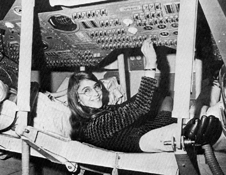
\includegraphics[scale=.6]{img/margaret-in-action.png}      

      \vfill
      {\tiny Fonte: \href{https://en.wikipedia.org/wiki/File:Margaret_Hamilton.gif}{NASA}}
  
  \end{column}
\only<2>{
    \begin{column}{.5\textwidth}
      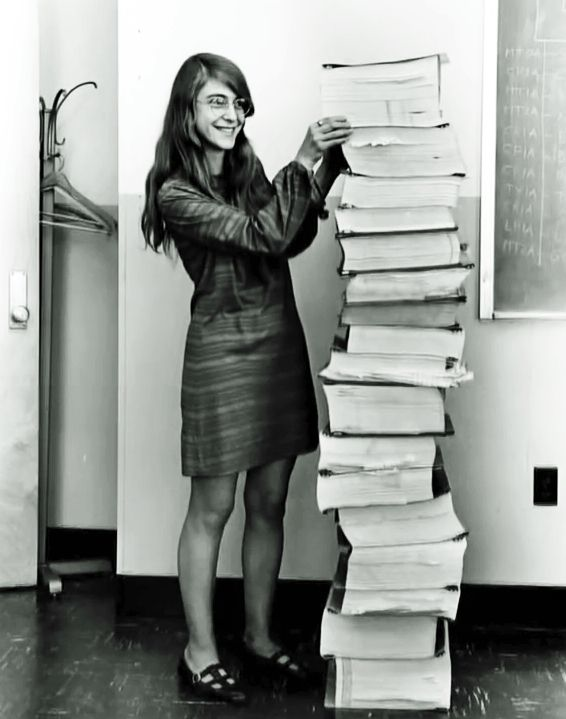
\includegraphics[scale=.22]{img/margaret.png}

      \vfill
      {\tiny Fonte: NASA via \href{https://en.wikipedia.org/wiki/File:Margaret_Hamilton.gif}{Wikipedia}}      
    \end{column}
}
  \end{columns}

\end{frame}

\begin{frame}{Referências}
  \begin{thebibliography}{1}

  \bibitem{brooks1975}
    Frederick~{P.}\ Brooks.
    \newblock {\em The Mythical Man-Month}.
    \newblock Addison-Wesley, 1975.
    
  \bibitem{humble:dijkstra1972}
    Edsger~W. Dijkstra.
    \newblock The humble programmer.
    \newblock {\em Communication of the ACM}, 15(10):859--866, 1972.

  \end{thebibliography}

\end{frame}

%% 
% Local variables:
% mode: latex
% mode:auto-fill
% TeX-file: main
% End:
%%

%% Fonte: http://users.csc.calpoly.edu/~jdalbey/205/Lectures/myths.html

\lecture{Mitos de Desenvolvimento de Software}{myths}

\lecturetitle{\course}{\insertlecture}

\section*{\insertlecture}

\frame{\maketitle}

\begin{frame}{Mítico Homêm-Mês}
\footnotesize
  \begin{columns}
    \begin{column}{.4\textwidth}
      
\includegraphics[scale=.35]{img/mitico.png}
    \end{column}
    \begin{column}{.6\textwidth}
      \begin{itemize}
      \item Observações do autor sobre a experiência de desenvolvimento 
        do sistema operacional OS/360 (1964--*) na IBM.
      \item 1$^a$ publicação: 1975.
      \end{itemize}
    \end{column}

  \end{columns}
  
\end{frame}

\begin{frame}{\inserttitle}

Os mitos são classificados de acordo com o ponto de vista de quem 
os emprega em mitos de:

  \begin{enumerate}[<+-| alert@+>]
  \item Gerenciamento;
  \item Desenvolvimento;
  \item Desenvolvedor.
  \end{enumerate}

\end{frame}

\note{A seguir são descritos alguns mitos que normalmente conduzem à
produção de software com defeitos, atraso na entrega ou cancelamento
do projeto. Os mitos foram classificados de acordo com o ponto de
vista de quem os emprega.}

\begin{frame}{Mitos de Gerenciamento}
\small
\begin{description}[<+-| alert@+>]
\item[Normas e padrões] Normas são editadas por empresas e comitês, às
  vezes são úteis. Porém, podem se tornar irrelevantes, incompletas e
  incompreensíveis se não estiverem vinculadas à realidade.
\item[Ferramentas] Ferramentas podem ajudar, porém não fazem mágica. A
  solução de problemas requerem mais que ferramentas, requerem um
  profundo entendimento do problema e da solução. Segundo Fred
  Brooks~\cite{brooks1975}, não há ``bala de prata'' no
  desenvolvimento de software.
\item[Mais programadores:] A solução intuitiva de que adicionando mais
  programadores pode fazer com que um projeto cumpra seu prazo é
  completamente errônea. Este procedimento causa sobrecarga de
  comunicação e atraso devido ao tempo que os novos integrantes da
  equipe leva para entender o problemas e solução. Segundo Fred
  Brooks~\cite{brooks1975}, ``adicionando pessoas a um projeto
  atrasado torna-o mais atrasado''.
\end{description}

\end{frame}

\begin{frame}{Mitos de Desenvolvimento}

\begin{description}[<+-| alert@+>]
\item[Alterações são fáceis:] Alterações em um software não são
  facilmente acomodadas como a princípio parecem ser. As alterações
  podem tornar o software mais complexo, introduzir novos erros e
  exigir uma quantidade enorme de trabalho devido às modificações em
  todos os processos relacionados (teste, documentação, $\ldots$).

\item[Visão superficial:] {\bf Uma visão geral da solução é suficiente
    para começar a programar.} É necessário um visão concreta sobre os
  requisitos, para detalhar os problemas e soluções para dar início ao
  desenvolvimento.
\end{description}

\end{frame}

\begin{frame}{Mitos do Desenvolvedor}

\begin{itemize}[<+-| alert@+>]
\item {\bf O trabalho acaba quando o programa é entregue:} O software requer
  atenção após a entrega, a manutenção, aperfeiçoamento e extensões
  geram uma necessidade contínua de suporte.
\item {\bf O sucesso de um projeto depende somente da qualidade do software
  entregue:} Documentação e informações de configuração são
  extremamente importantes.
\item {\bf Não há como avaliar a qualidade de um software até que ele
  esteja executando:} Devido a natureza abstrata do software, ele pode
  ser avaliado sem que uma linha de código seja produzida. Há métodos
  formais de análise para verificação de pontos críticos com relação à
  corretude, segurança e confiabilidade.
\end{itemize}

\end{frame}

\begin{frame}{Referências}
\bibliographystyle{plain}
\bibliography{software-engineering}
\end{frame}


%%
% Local variables:
% mode: latex
% mode:auto-fill
% TeX-file: main
% End:
%%

%\lecture{Metodologias de Desenvolvimento de Software}{methods}

\lecturetitle{\course}{\insertlecture}

\frame{\maketitle}

\section{Princípios da Engenharia de Software}

\begin{frame}{Princípios de desenvolvimento de software/sistemas}

  \begin{description}[<+-| alert@+>]
  \item[Formalização:] aplicação de métodos formais para aumento da
    confiabilidade;
  \item[Abstração:] representação do mundo real com nível de
    detalhamento adequado para eliminação da complexidade;
  \item[Decomposição:] divisão em partes menores para redução 
    da complexidade;
  \item[Generalização:] descoberta ou adoção de princípios
    fundamentais que permitem reutilização;
  \item[Flexibilização:] adaptação è evolução, extensão e
    aperfeiçoamento.
  \end{description}
  
\end{frame}

\section{Ciclo de vida do software}
  
\begin{frame}{Ciclo de vida do software}

\input{img/lifecycle}

\end{frame}


\begin{frame}{Desenvolvimento em Cascata}

\input{img/waterfall-method}  

\end{frame}

\begin{frame}{Método Evolutivo}
  \begin{center}
  \begin{tikzpicture}
    [font=\scriptsize,phase/.style={minimum height=1cm,draw},
    protophase/.style={minimum width=3cm,ellipse,draw},
    version/.style={white,fill=black,circle,draw},
    every path/.style={->,>=latex,draw}]

    \node[phase,tape,thick] (requirements) {Requisitos};
    \node[thick,minimum height=5cm,minimum width=3.2cm,draw] (prototype) [right of=requirements,xshift=2cm] {};
    \node[above] at (prototype.north) {Prototipação};
    \node[fill=yellow,protophase] (dev) [right of=requirements,xshift=2cm,yshift=1cm]
    {Implementação};
    \node[fill=gray,protophase] (eval) [right of=requirements,xshift=2cm,yshift=-1cm]  {Validação};
    
    \node[version] (v0) [right of=prototype,xshift=2cm,yshift=2.5cm] {Versão
      0};
    \node[version] (v1) [right of=prototype,xshift=2cm]
    {Versão 1};
    \node[]  [right of=prototype,xshift=2cm,yshift=-1.25cm] {$\vdots$};
    \node[version] (vN) [right of=prototype,xshift=2cm,yshift=-2.5cm] {Versão N};

    \path (requirements) -> (prototype);
    \path (dev.south west) -> (eval.north west);
    \path (eval.north east) -> (dev.south east);
    \path (prototype.north east) -> (v0);
    \path (prototype.east) -> (v1);
    \path (prototype.south east) -> (vN);
  \end{tikzpicture}
\end{center}

\end{frame}


\begin{frame}{Método Evolutivo}

\begin{block}{Vantagens}
  \begin{itemize}[<+-| alert@+>]\setbeamercovered{transparent}
  \item Verificação antecipada de possíveis problemas durante a
    implementação: linguagem de programação, algoritmo, performance.
  \item Maior interação com o cliente, permitindo esclarecer dúvidas
    sobre requisitos que não estejam bem definidos.
  \end{itemize}
\end{block}  

\end{frame}

\begin{frame}{Método Evolutivo}

\begin{block}{Desvantagens}
  \begin{itemize}[<+-| alert@+>]\setbeamercovered{transparent}

    \item Não é dada atenção à documentação, pois cada protótipo é
      visto como provisório.

  \item Pode causar inconsistências na estrutura do projeto.
    \note{Envolve o mito de que alterações são fáceis}

    \item Dá a impressão ao cliente, em algumas versões, de que o
      projeto está quase pronto.
      \note{O cliente irá pressionar para usá-lo, achando que somente
        algumas alterações são necessárias}

    \item O desenvolvedor pode fazer escolhas inapropriadas para
      adiantar um protótipo, prejudicando as versões seguintes.
  \end{itemize}
\end{block}

\end{frame}


\begin{frame}{Método Espiral}{Boehm}
  
  \begin{block}{Características}
    \begin{itemize}[<+-| alert@+>]\setbeamercovered{transparent}
    \item Incorpora características dos processos em cascata e
      evolutivo, com a adição da análise de risco.
      \note{Dá atenção especial às partes críticas do projeto}
    \item Cada iteração da espiral se beneficia das lições da anterior.
    \item O protótipo está mais voltado para o projeto e não para o
      funcionamento do sistema.
      \note{Evita expectativas do cliente com relação ao programa.}
      \item Mais flexível que o cascata;
      \item O protótipo não é funcional, o que provoca riscos em caso
        de pressão para produzir algo ou corte de gastos;
    \end{itemize}
  \end{block}
\end{frame}


\begin{frame}{Método Espiral}

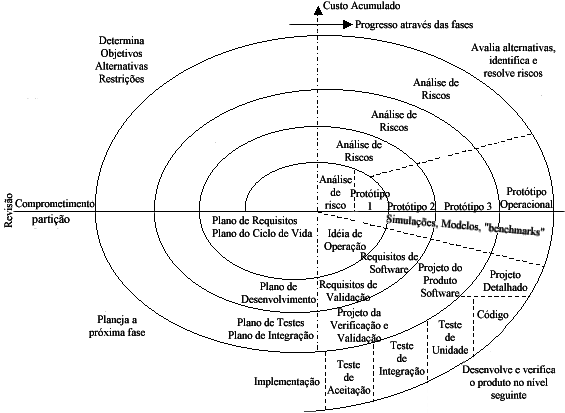
\includegraphics[scale=.4]{img/spiral.png}

\vfill
{\tiny Fonte: \href{http://www2.dem.inpe.br/ijar/CicoloVidaSoftPrado.html}{Engenharia de Software, Capítulo 2 - Ciclo de Vida do Software, Professor Prado.}}
\end{frame}


\lecture{Rational Unified Process (RUP)}{RUP}

\begin{frame}{\insertlecture}
  Processo baseado na UML ({\em Unified Modeling Language}) criado
  pela Rational Corp., adquirida pela IBM. O processo baseia-se nas
  fases conforme a figura a seguir:

  \begin{center}
    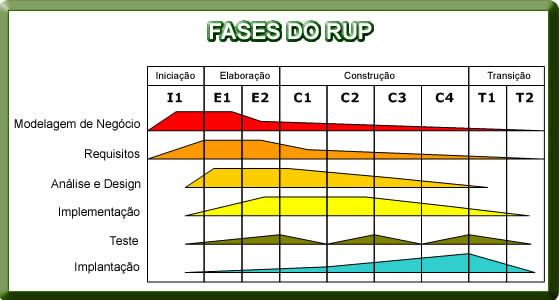
\includegraphics[scale=.6]{img/fasesRUP.png}\\
    {\tiny Fonte: \href{https://www.infoescola.com/engenharia-de-software/rup/}{RUP. Marina Martinez.}}
  \end{center}
\end{frame}

\begin{frame}{\insertlecture}{Fases}
  \begin{enumerate}[<+-| alert@+>]\setbeamercovered{transparent}
  \item {\bf Concepção/Iniciação}: define o escopo do projeto,
    cronograma e despesas. É usado para verificar o progresso.
  \item {\bf Elaboração}: trabalho com o cliente para identificar
    casos de uso, projeta a arquitetura de software, ajusta o plano de
    desenvolvimento e constrói um protótipo inicial.
  \item {\bf Construção}: codifica e testa o produto, resultando no
    primeiro lançamento de teste.
  \item {\bf Transição}: move o produto do ambiente de desenvolvimento
    para o ambiente de produção, onde inclui o teste de aceitação do
    cliente e o treinamento do usuário.
  \end{enumerate}
\end{frame}

\begin{frame}{\insertlecture}{\em Workflows}
  \begin{enumerate}[<+-| alert@+>]\setbeamercovered{transparent}
  \item Modelagem de negócio;
  \item Requisitos;
  \item Análise e especificação/design;
  \item Implementação;
  \item Teste;
  \item Implantação.
  \end{enumerate}
\end{frame}

\begin{frame}{\insertlecture}{Considerações}
  \begin{itemize}
  \item Diferente do Cascata, cada fase do RUP envolve iteração. Por
    exemplo, a concepção pode ter uma iteração, a elaboração duas, a
    construção quatro e a transição duas. Como o Espiral, o RUP pode
    iterar através das quatro fases repetidamente.
  \end{itemize}  
\end{frame}

\begin{frame}{Abordagem de Planejar-Documentar}
  \begin{itemize}[<+-| alert@+>]\setbeamercovered{transparent}
  \item O métodos e processos vistos exigem uma abordagem
    que envolve Planejamento e documentação, por isso, são considerados
    mais pesados do que as abordagens Ágeis.
  \item Alguns programadores consideram estas metodologias tediosas 
    para o desenvolvimento de software.
  \end{itemize}
\end{frame}

% \begin{frame}{Métodos ágeis}
  
%   \begin{block}{Características}
%     \begin{itemize}[<+->]
%     \item Código como principal medida de progresso;
%     \item Colaboração entre desenvolvedores e clientes que participam
%       mais ativamente das fases de desenvolvimento;
%     \item Comunicação frequente;
%     \item Simplificação da documentação;
%     \item Testes como guias para o desenvolvimento;
%     \item Desenvolvimento em pequenos incrementos com integração contínua;
%     \item Práticas como programação em grupos de duas pessoas.
%       \note{Para aumentar o número de pessoas pensando sobre as
%         decisões técnicas e capturar erros mais facilmente.}
%     \end{itemize}
%   \end{block}
% \end{frame}


\begin{frame}{Referência}
  \begin{itemize}
  \item {\color{blue}''Engineering Software as a Service: An Agile Approach Using
    Cloud Computing.''} Armando Fox,‎ David Patterson. Strawberry Canyon
    LLC, 2014.
  \end{itemize}  
\end{frame}
%\lecture{Levantamento e Análise de Requisitos}{requirements}

\lecturetitle{\course}{\insertlecture}

\section{\insertlecture}

\frame{\maketitle}

\begin{frame}{\insertlecture}
  
  \begin{itemize}[<+->]\setbeamercovered{transparent}
  \item O software deve se adaptar às necessidades dos usuários;
    \begin{itemize}
    \item As melhores técnicas de programação---algoritmos, estrutura de dados, 
      análise de performance, estrutura modular---não salvarão o projeto da falha.
    \end{itemize}
  \item Os softwares são construídos para atender os clientes, em especial os usuários, 
    e devem se adaptar às suas necessidades.
  \end{itemize}

  \pause
  
  O levantamento e análise de requisitos tenta atingir um equilíbrio
  entre o que os usuários querem e o que o sistema fará.
  \note{Equilíbrio porque alguma negociação deve haver.}

\end{frame}

\begin{frame}{Produtos da fase requisitos}
  \begin{description}[<+->]\setbeamercovered{transparent}
  \item[Documento de requisitos] descrevendo as características do
    software a ser construído.
  \item[Plano de validação] descrevendo como o futuro software, uma
    vez construído, será testado.
  \end{description}
\end{frame}

\begin{frame}{O Padrão IEEE}
  \begin{itemize}
  \item
    \href{http://holanda.xyz/files/720574.pdf}{Prática
      Recomendada para as Especificações de Requisitos de
      Software. IEEE Computer Society. IEEE Std 830-1998.}

    \begin{itemize}
    \item Conjunto de listas para checagem de propriedades que o sistema
      deve satisfazer.
    \end{itemize}
    \note{O padrão ajuda a levantar as propriedades, tentando antecipar
      problemas que poderiam ocorrer.}
  \end{itemize}
\end{frame}

\begin{frame}{Escopo dos Requisitos}
  \begin{description}[<+->]\setbeamercovered{transparent}
  \item[Requisitos Funcionais] definem as funções que o sistema deve
    possuir. Possuem entrada, processamento e saída.
  \item[Requisitos Não-Funcionais] performance, portabilidade, éticos,
    legais, integração.
  \end{description}
\end{frame}

\begin{frame}{Obtendo os Requisitos}
  
  A obtenção dos requisitos é uma {\bf negociação} entre as propriedades
  desejadas pelo usuário para o sistema e as possibilidades de
  desenvolvimento e custos expostas pela equipe técnica.

  \pause

  \begin{block}{Principais fatores a serem equilibrados}
  \begin{itemize}[<+->]\setbeamercovered{transparent}
  \item Alguns usuários têm visões conflitantes sobre o sistema;
  \item Algumas propriedades desejadas são inviáveis em termos de custo ou 
    desenvolvimento;
  \item Os usuários tendem a pensar em termos de sistemas existentes;
  \item Fatores externos afetam a escolha das funcionalidades,
    principalmente, custo e interferência da instituição onde o
    sistema será implantado.
  \end{itemize}
\end{block}

\end{frame}

\begin{frame}{Técnicas para levantamento de requisitos}
  \begin{itemize}[<+->]\setbeamercovered{transparent}
  \item Entrevistas;
  \item Workshops;
  \item Sistemas anteriores;
  \item Sistemas similares.
  \end{itemize}
\end{frame}

\frame{\author{}\date{}\title{Documentação de requisitos}\maketitle}

\subsection{Documentação de requisitos}

\begin{frame}{Documentação dos requisitos}
  Formas de escrever uma especificação de requisitos do sistema:

  \begin{description}[<+->]\setbeamercovered{transparent}
  \item[Sentenças em linguagem natural:] Os requisitos são escritos em forma de frases.
  \item[Linguagem natural estruturada:] Os requisitos são escritos em um formulário.
    \item[Notações gráficas:] Utiliza figuras e diagramas com texto associado.
  \item[Especificações matemáticas:] Usa notações matemáticas, como máquina de estados 
    finitos e teoria de conjuntos.
  \end{description}
\end{frame}

\begin{frame}{Sentenças em linguagem natural}
  Exemplo de requisitos funcionais de um sistema de gestão de pessoas, disciplinas e notas 
  de uma Faculdade ou Universidade:
  \begin{enumerate}
  \item Cadastro de pessoas por funcionários da Faculdade.
    \item Consulta de pessoas por funcionários da Faculdade.
    \item Cadastro de disciplinas por funcionário da Faculdade. 
    \item Inserção de notas por professores.
    \item Consulta de notas por parte dos alunos.
    \end{enumerate}
\end{frame}

\begin{frame}{Linguagem natural estruturada}

  {\bf Sistema de gerenciamento para Faculdade ou Universidade}\\\bigskip

  \begin{tabular}[h]{|l|l|}\hline
    \bf Função: & Gerenciar dados de pessoas, disciplinas e notas.\\\hline
    \bf Descrição: & O sistema deve armazenar os dados de funcionários, \\
    & alunos e docentes, de disciplinas e de notas.\\\hline
    \bf Entradas: & Pessoas: nome, endereço, RG, CPF.\\
                & Disciplinas: nome, responsável, resumo.\\
                & Notas: nome da disciplina, nome do aluno, valor.\\\hline
    \bf Saídas: & Visualização das entradas.\\\hline
    
  \end{tabular}
\end{frame}

\begin{frame}{Notação gráfica}
  
  Exemplo de uso de notação gráfica para a documentação de requisitos, no 
  caso, diagrama de casos de uso da UML ({\em Unified Modeling Language}):

  \begin{center}
    \includegraphics[scale=.35]{usecase.png}
  \end{center}

\end{frame}

\begin{frame}{Especificações matemáticas}
  
  Especificação do sistema de uma catraca usando máquina de estados finitos:\bigskip
\begin{center}
  \includegraphics[scale=.35]{state.png}
\end{center}
\end{frame}

\begin{frame}[fragile]{Especificações matemáticas, continuação}

  Especificação de um relógio binário usando a lógica temporal de ações (TLA$^+$, \href{http://research.microsoft.com/en-us/um/people/lamport/tla/tla.html}{\em Temporal Logic of Actions}):

\begin{multline}
  \text{VARIABLE clock}\hfill\\
  \text{Init} \equiv clock \in \{0, 1\}\hfill\\
  \text{Tick} \equiv \text{IF}\ clock = 0\ \text{THEN}\ clock' = 1\ \text{ELSE}\ clock' = 0\hfill\\
  \text{Spec} \equiv \text{Init} \land [][\text{Tick}]_{\langle clock\rangle}\hfill
\end{multline}

\end{frame}

\begin{frame}{Referências}  
  \begin{enumerate}
  \item \ianref
  \item \pfref
  \item Bertrand Meyer, ``Touch of Class: Learning to Program Well
    with Objects and Contracts'', Springer, 2009.
  \end{enumerate}
\end{frame}
%\input viabilidade
\input project
%\input uml
%\input classes
%\input inheritance
%\input polymorphism
%\input generics

%\input quality
%\input cmmi
%\input spice
%\input metricas
\input agil

\input config
\input vcs
\input make
\input TDD
%\input refactoring
%\input formal
%\input tlaplus
\end{document}
"
% to turn off transitions
\ifdefined\ishandout
  \documentclass[handout]{beamer}
\else
  \documentclass[]{beamer}
\fi

\setbeamercovered{highly dynamic}
\newcounter{saveenumi}% save counter on enumerate across frames
\newcommand{\seti}{\setcounter{saveenumi}{\value{enumi}}}
\newcommand{\conti}{\setcounter{enumi}{\value{saveenumi}}}
\resetcounteronoverlays{saveenumi}

% Dependencies
\usepackage{fontspec} % use XeLaTeX
\usepackage[]{polyglossia}
\setdefaultlanguage{brazil}
% \usepackage{lcg} % Generate random numbers
\usepackage{hyperref}
\hypersetup{colorlinks=true,linkcolor=blue,anchorcolor=blue,urlcolor=blue}
\usepackage{pgf,tikz} % Draw figures
\usetikzlibrary{arrows,automata,calc,chains,circuits,graphs,positioning,shapes.gates.logic.US,shapes,trees}
\usepackage{circuitikz}
%\usepackage{pgfgantt}
  % \usepackage{pgfplots}
  % \usegdlibrary{trees}
  \usepackage{listings}
  \lstset{language=C,inputencoding=utf8,basicstyle=\footnotesize, 
    flexiblecolumns=true, numbers=left, numberstyle=\tiny\color{gray}, 
    commentstyle=\scriptsize\color{black!50},mathescape}
  \usepackage{pdftexcmds} % \pdf@strcmp \pdf@filemoddate
  \usepackage{ifthen} % \ifthenelse
  \usepackage{animate}

  % FONTS
  \font\fiverm=cmr5
  \font\ninerm=cmr9

  % Definitions
  \author{Adriano J. Holanda}%\\{\scriptsize \url{http://holanda.xyz}}}
  \def\array{vetor}
  \def\bigO#1{\mathcal{O}(#1)}
  \def\bug#1{{\it bug#1\/}}
  % C letter
  \font\ninerm=cmr9
  \let\mc=\ninerm
  \def\CEE{{\mc C\spacefactor1000}}

  \def\boxset{
    \tikzset{box/.style={rectangle,minimum width=.5cm,draw},
      index/.style={minimum width=.5cm}}
  }

  % only title frames
  \def\onlytitleframe#1{\author{}\date{}\title{#1}\maketitle}

  % THEOREM
  % \newtheorem{teorema}[theorem]{Teorema}

  \newcommand{\executeiffilenewer}[3]{%
    \ifnum\pdf@strcmp{\pdf@filemoddate{#1}}%
    {\pdf@filemoddate{#2}}>0%
    {\immediate\write18{#3}}\fi%
  }
  % includesvg[includegraphics args]{file} command (linux-version)
  \newcommand{\includesvg}[2][]{%
    \executeiffilenewer{#2.svg}{#2.pdf}{%
      /usr/bin/inkscape -z -C --file="#2.svg" --export-pdf="#2.pdf" > /tmp/#2.log}%
    \ifthenelse{\equal{#1}{}}{%
      \includegraphics{#2}}{%
      \includegraphics[#1]{#2}}%
  }

\def\lecturetitle#1#2{\title{{\large\bf#1}\\{\small [#2]}}}

\def\transitionslide#1{\frame{\author{}\title{\LARGE#1}\date{}\maketitle}}

  \def\shcmd#1{
    \begingroup
    \bigskip\color{gray}
    {\tt \$~#1}
    \bigskip
    \endgroup
  }


  \def\fonte#1{\begingroup\tiny\tt\color{gray} Fonte:~#1\endgroup}

\usepackage{amsmath}
\usepackage{pgf-umlcd}
\usepackage{listings}
\lstset{    
  columns=flexible,
  basicstyle=\scriptsize,
  commentstyle={\scriptsize\color{gray}},
  numbers=left,numberstyle=\tiny,numbersep=5pt,
  frame=single,
  language=Java}

\usefonttheme{professionalfonts}

\def\ianref{Ian Sommerville. ``Engenharia de Software''. Editora Pearson, 9$^a$~edição, 2011.}
\def\ariadneref{Ariadne M. B. R. Carvalho, Thelma C. S. Chiossi. ``Introdução à Engenharia de Software''. Editora UNICAMP, 2001.}

\def\pfref{S. L. Pfleeger. ``Engenharia de Software: Teoria e Prática''. Editora Pearson, 2$^a$ edição, 2004.}

\def\oopimgdir{~/holanda.git/edu/oop/img}

\def\course{Engenharia de Software}

\begin{document}
\date{\today}

%\lecture{Introdução}{intro}

\lecturetitle{\course}{\insertlecture}

\frame{\maketitle}

\section*{\insertlecture}



% \begin{frame}{O que é Engenharia de Software}
  
%   \begin{description}
%   \item[Engenharia:]
%     \href{http://www.thefreedictionary.com/engineering}{Aplicação dos
%       princípios {\bf matemáticos} e {\bf científicos} para fins práticos tais
%       como o projeto, manufatura e operação de estruturas, máquinas,
%       processos e sistemas {\bf eficientes} e {\bf econômicos}.}

%   \item[Software:]~conjunto de instruções para o computador para
%     executar tarefas e manipular dados.

%   \item[Engenharia de Software:]~Aplicação dos princípios {\bf
%       matemáticos} e {\bf científicos} para o projeto, implementação e
%     operação de conjunto de instruções para o computador.
%   \end{description}

% \end{frame}

% \begin{frame}{O que é Engenharia de Software}

%   \note{A definição apresentada não é totalmente aplicável à Engenharia de
%   Software, pois, alguns projetos aplicam métodos de produção
%   empíricos, ou seja, baseados na experiência.}
  
%   Uma definição mais
%   adequada é a formulada por Carvalho \& Chiossi~\cite{carvalho2001},
%   como sendo:

%   \begin{quote}
%     Uma disciplina que reúne metodologias, métodos e ferramentas a ser
%     utilizados, desde a percepção do problema até o momento em que o
%     sistema desenvolvido deixa de ser operacional, visando resolver
%     problemas inerentes ao processo de desenvolvimento e ao produto de
%     software.
%   \end{quote}
% \pause
%   Porém, o objetivo continua sendo o mesmo da Engenharia, tornar o
%   processo de produção de software eficiente e econômico.

% \end{frame}

\begin{frame}{Crise do Software}

  A ineficiência dos softwares e atrasos constantes de entrega,
  tornando-os financeiramente custosos, produziu o termo ``Crise do
  Software'', cunhado em 1968 durante a Conferência de Engenharia de
  Software da OTAN (Organização do Tratado do Atlântico Norte)
  realizada na Alemanha. Segundo Dijkstra, esta crise está relacionada
  ao aumento do poder de processamento das
  máquinas~\cite{humble:dijkstra1972}.

\end{frame}

%%% Matéria sobre a Apollo 11
% https://qz.com/726338/the-code-that-took-america-to-the-moon-was-just-published-to-github-and-its-like-a-1960s-time-capsule/

\begin{frame}{Software de controle de navegação: Apollo~11 (1969)}
  \footnotesize
  \begin{itemize}
  \item Tempo de desenvolvimento: 1961--1972.
  \item Coordenação: Margaret Hamilton, MIT.
  \item Linguagem: Assembly. O código fonte está disponível em  \url{https://github.com/chrislgarry/Apollo-11/}.
  \end{itemize}

  \begin{columns}
    \begin{column}{.5\textwidth}
     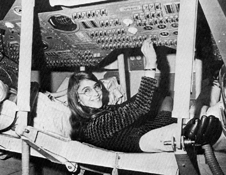
\includegraphics[scale=.6]{img/margaret-in-action.png}      

      \vfill
      {\tiny Fonte: \href{https://en.wikipedia.org/wiki/File:Margaret_Hamilton.gif}{NASA}}
  
  \end{column}
\only<2>{
    \begin{column}{.5\textwidth}
      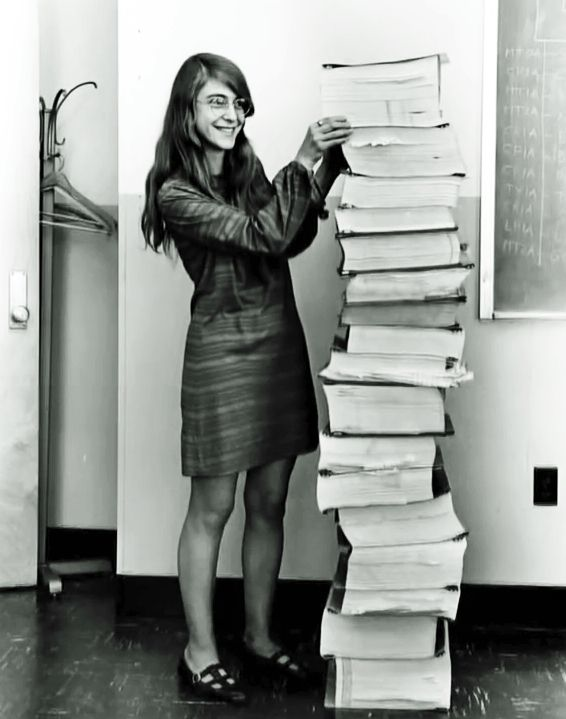
\includegraphics[scale=.22]{img/margaret.png}

      \vfill
      {\tiny Fonte: NASA via \href{https://en.wikipedia.org/wiki/File:Margaret_Hamilton.gif}{Wikipedia}}      
    \end{column}
}
  \end{columns}

\end{frame}

\begin{frame}{Referências}
  \begin{thebibliography}{1}

  \bibitem{brooks1975}
    Frederick~{P.}\ Brooks.
    \newblock {\em The Mythical Man-Month}.
    \newblock Addison-Wesley, 1975.
    
  \bibitem{humble:dijkstra1972}
    Edsger~W. Dijkstra.
    \newblock The humble programmer.
    \newblock {\em Communication of the ACM}, 15(10):859--866, 1972.

  \end{thebibliography}

\end{frame}

%% 
% Local variables:
% mode: latex
% mode:auto-fill
% TeX-file: main
% End:
%%

%% Fonte: http://users.csc.calpoly.edu/~jdalbey/205/Lectures/myths.html

\lecture{Mitos de Desenvolvimento de Software}{myths}

\lecturetitle{\course}{\insertlecture}

\section*{\insertlecture}

\frame{\maketitle}

\begin{frame}{Mítico Homêm-Mês}
\footnotesize
  \begin{columns}
    \begin{column}{.4\textwidth}
      
\includegraphics[scale=.35]{img/mitico.png}
    \end{column}
    \begin{column}{.6\textwidth}
      \begin{itemize}
      \item Observações do autor sobre a experiência de desenvolvimento 
        do sistema operacional OS/360 (1964--*) na IBM.
      \item 1$^a$ publicação: 1975.
      \end{itemize}
    \end{column}

  \end{columns}
  
\end{frame}

\begin{frame}{\inserttitle}

Os mitos são classificados de acordo com o ponto de vista de quem 
os emprega em mitos de:

  \begin{enumerate}[<+-| alert@+>]
  \item Gerenciamento;
  \item Desenvolvimento;
  \item Desenvolvedor.
  \end{enumerate}

\end{frame}

\note{A seguir são descritos alguns mitos que normalmente conduzem à
produção de software com defeitos, atraso na entrega ou cancelamento
do projeto. Os mitos foram classificados de acordo com o ponto de
vista de quem os emprega.}

\begin{frame}{Mitos de Gerenciamento}
\small
\begin{description}[<+-| alert@+>]
\item[Normas e padrões] Normas são editadas por empresas e comitês, às
  vezes são úteis. Porém, podem se tornar irrelevantes, incompletas e
  incompreensíveis se não estiverem vinculadas à realidade.
\item[Ferramentas] Ferramentas podem ajudar, porém não fazem mágica. A
  solução de problemas requerem mais que ferramentas, requerem um
  profundo entendimento do problema e da solução. Segundo Fred
  Brooks~\cite{brooks1975}, não há ``bala de prata'' no
  desenvolvimento de software.
\item[Mais programadores:] A solução intuitiva de que adicionando mais
  programadores pode fazer com que um projeto cumpra seu prazo é
  completamente errônea. Este procedimento causa sobrecarga de
  comunicação e atraso devido ao tempo que os novos integrantes da
  equipe leva para entender o problemas e solução. Segundo Fred
  Brooks~\cite{brooks1975}, ``adicionando pessoas a um projeto
  atrasado torna-o mais atrasado''.
\end{description}

\end{frame}

\begin{frame}{Mitos de Desenvolvimento}

\begin{description}[<+-| alert@+>]
\item[Alterações são fáceis:] Alterações em um software não são
  facilmente acomodadas como a princípio parecem ser. As alterações
  podem tornar o software mais complexo, introduzir novos erros e
  exigir uma quantidade enorme de trabalho devido às modificações em
  todos os processos relacionados (teste, documentação, $\ldots$).

\item[Visão superficial:] {\bf Uma visão geral da solução é suficiente
    para começar a programar.} É necessário um visão concreta sobre os
  requisitos, para detalhar os problemas e soluções para dar início ao
  desenvolvimento.
\end{description}

\end{frame}

\begin{frame}{Mitos do Desenvolvedor}

\begin{itemize}[<+-| alert@+>]
\item {\bf O trabalho acaba quando o programa é entregue:} O software requer
  atenção após a entrega, a manutenção, aperfeiçoamento e extensões
  geram uma necessidade contínua de suporte.
\item {\bf O sucesso de um projeto depende somente da qualidade do software
  entregue:} Documentação e informações de configuração são
  extremamente importantes.
\item {\bf Não há como avaliar a qualidade de um software até que ele
  esteja executando:} Devido a natureza abstrata do software, ele pode
  ser avaliado sem que uma linha de código seja produzida. Há métodos
  formais de análise para verificação de pontos críticos com relação à
  corretude, segurança e confiabilidade.
\end{itemize}

\end{frame}

\begin{frame}{Referências}
\bibliographystyle{plain}
\bibliography{software-engineering}
\end{frame}


%%
% Local variables:
% mode: latex
% mode:auto-fill
% TeX-file: main
% End:
%%

%\lecture{Metodologias de Desenvolvimento de Software}{methods}

\lecturetitle{\course}{\insertlecture}

\frame{\maketitle}

\section{Princípios da Engenharia de Software}

\begin{frame}{Princípios de desenvolvimento de software/sistemas}

  \begin{description}[<+-| alert@+>]
  \item[Formalização:] aplicação de métodos formais para aumento da
    confiabilidade;
  \item[Abstração:] representação do mundo real com nível de
    detalhamento adequado para eliminação da complexidade;
  \item[Decomposição:] divisão em partes menores para redução 
    da complexidade;
  \item[Generalização:] descoberta ou adoção de princípios
    fundamentais que permitem reutilização;
  \item[Flexibilização:] adaptação è evolução, extensão e
    aperfeiçoamento.
  \end{description}
  
\end{frame}

\section{Ciclo de vida do software}
  
\begin{frame}{Ciclo de vida do software}

\begin{tikzpicture}
  [cycle/.style={text centered,text width=2.75cm,minimum width=2cm,
    minimum height=1.5cm,draw},every path/.style={->,>=latex,draw}]
  \def\D{2cm}

  \node<1->[cycle,blue] (spec) {Levantamento e Análise de Requisitos};
  \node<2->[cycle,green!40!black] (proj) [below of=spec,yshift=-\D] {Projeto: Especificação, Modelagem};
  \node<3->[cycle] (dev) [right of=proj,xshift=3.25*\D] {Implementação e Testes};
  \node<4->[cycle,red] (deploy) [above of=dev,yshift=\D] {Implantação e Validação};
  \node<5->[cycle,brown] (maintain) [left of=deploy,xshift=-1.15*\D] {Manutenção};
  
  \path<2-> (spec) -- (proj);
  \path<3-> (proj) -- (dev);
  \path<4-> (dev) -- (deploy);
  \path<5-> (deploy) -- (maintain);
\end{tikzpicture}

%%
% Local variables:
% mode: latex
% End:
%%

\end{frame}


\begin{frame}{Desenvolvimento em Cascata}

\begin{tikzpicture}
  [font={\tiny\bf},node distance=2.25cm,every path/.style={->,>=latex,draw},
  cycle/.style={thick,rounded corners=3mm,text centered,text width=1.5cm,minimum width=1cm, minimum
    height=1.5cm,draw},
  dev/.style={cycle},
  deploy/.style={cycle,red},
  maintain/.style={cycle,brown!40!black}]

  \node<1->[cycle,blue] (requirements) {Levantamento e Análise de Requisitos};
  \node<2->[cycle,green!40!black] (proj) [right of=requirements,yshift=-1cm] {Projeto: Especificação, Modelagem};
  \node<3->[dev] (dev) [right of=proj,yshift=-1cm] {Implementação e Testes};
  \node<4->[deploy] (deploy) [right of=dev,yshift=-1cm] {Implantação e Validação};
  \node<5->[maintain] (maintain) [right of=deploy,yshift=-1cm] {Manutenção};
  
  \path<2-> (requirements) edge [bend left] (proj.north);
  \path<3-> (proj) edge [bend left]  (dev.north);
  \path<4-> (dev) edge [bend left]  (deploy.north);
  \path<5-> (deploy) edge [bend left]  (maintain.north);
\end{tikzpicture}
  

\end{frame}

\begin{frame}{Método Evolutivo}
  \begin{center}
  \begin{tikzpicture}
    [font=\scriptsize,phase/.style={minimum height=1cm,draw},
    protophase/.style={minimum width=3cm,ellipse,draw},
    version/.style={white,fill=black,circle,draw},
    every path/.style={->,>=latex,draw}]

    \node[phase,tape,thick] (requirements) {Requisitos};
    \node[thick,minimum height=5cm,minimum width=3.2cm,draw] (prototype) [right of=requirements,xshift=2cm] {};
    \node[above] at (prototype.north) {Prototipação};
    \node[fill=yellow,protophase] (dev) [right of=requirements,xshift=2cm,yshift=1cm]
    {Implementação};
    \node[fill=gray,protophase] (eval) [right of=requirements,xshift=2cm,yshift=-1cm]  {Validação};
    
    \node[version] (v0) [right of=prototype,xshift=2cm,yshift=2.5cm] {Versão
      0};
    \node[version] (v1) [right of=prototype,xshift=2cm]
    {Versão 1};
    \node[]  [right of=prototype,xshift=2cm,yshift=-1.25cm] {$\vdots$};
    \node[version] (vN) [right of=prototype,xshift=2cm,yshift=-2.5cm] {Versão N};

    \path (requirements) -> (prototype);
    \path (dev.south west) -> (eval.north west);
    \path (eval.north east) -> (dev.south east);
    \path (prototype.north east) -> (v0);
    \path (prototype.east) -> (v1);
    \path (prototype.south east) -> (vN);
  \end{tikzpicture}
\end{center}

\end{frame}


\begin{frame}{Método Evolutivo}

\begin{block}{Vantagens}
  \begin{itemize}[<+-| alert@+>]\setbeamercovered{transparent}
  \item Verificação antecipada de possíveis problemas durante a
    implementação: linguagem de programação, algoritmo, performance.
  \item Maior interação com o cliente, permitindo esclarecer dúvidas
    sobre requisitos que não estejam bem definidos.
  \end{itemize}
\end{block}  

\end{frame}

\begin{frame}{Método Evolutivo}

\begin{block}{Desvantagens}
  \begin{itemize}[<+-| alert@+>]\setbeamercovered{transparent}

    \item Não é dada atenção à documentação, pois cada protótipo é
      visto como provisório.

  \item Pode causar inconsistências na estrutura do projeto.
    \note{Envolve o mito de que alterações são fáceis}

    \item Dá a impressão ao cliente, em algumas versões, de que o
      projeto está quase pronto.
      \note{O cliente irá pressionar para usá-lo, achando que somente
        algumas alterações são necessárias}

    \item O desenvolvedor pode fazer escolhas inapropriadas para
      adiantar um protótipo, prejudicando as versões seguintes.
  \end{itemize}
\end{block}

\end{frame}


\begin{frame}{Método Espiral}{Boehm}
  
  \begin{block}{Características}
    \begin{itemize}[<+-| alert@+>]\setbeamercovered{transparent}
    \item Incorpora características dos processos em cascata e
      evolutivo, com a adição da análise de risco.
      \note{Dá atenção especial às partes críticas do projeto}
    \item Cada iteração da espiral se beneficia das lições da anterior.
    \item O protótipo está mais voltado para o projeto e não para o
      funcionamento do sistema.
      \note{Evita expectativas do cliente com relação ao programa.}
      \item Mais flexível que o cascata;
      \item O protótipo não é funcional, o que provoca riscos em caso
        de pressão para produzir algo ou corte de gastos;
    \end{itemize}
  \end{block}
\end{frame}


\begin{frame}{Método Espiral}

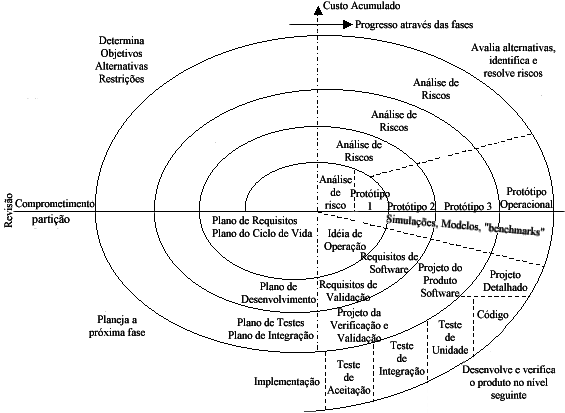
\includegraphics[scale=.4]{img/spiral.png}

\vfill
{\tiny Fonte: \href{http://www2.dem.inpe.br/ijar/CicoloVidaSoftPrado.html}{Engenharia de Software, Capítulo 2 - Ciclo de Vida do Software, Professor Prado.}}
\end{frame}


\lecture{Rational Unified Process (RUP)}{RUP}

\begin{frame}{\insertlecture}
  Processo baseado na UML ({\em Unified Modeling Language}) criado
  pela Rational Corp., adquirida pela IBM. O processo baseia-se nas
  fases conforme a figura a seguir:

  \begin{center}
    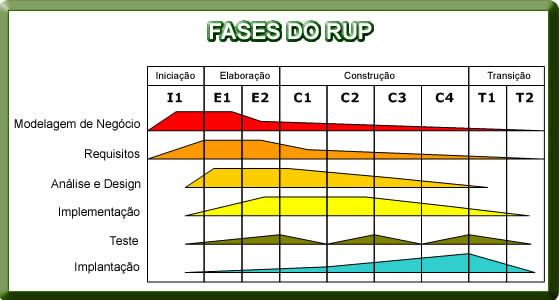
\includegraphics[scale=.6]{img/fasesRUP.png}\\
    {\tiny Fonte: \href{https://www.infoescola.com/engenharia-de-software/rup/}{RUP. Marina Martinez.}}
  \end{center}
\end{frame}

\begin{frame}{\insertlecture}{Fases}
  \begin{enumerate}[<+-| alert@+>]\setbeamercovered{transparent}
  \item {\bf Concepção/Iniciação}: define o escopo do projeto,
    cronograma e despesas. É usado para verificar o progresso.
  \item {\bf Elaboração}: trabalho com o cliente para identificar
    casos de uso, projeta a arquitetura de software, ajusta o plano de
    desenvolvimento e constrói um protótipo inicial.
  \item {\bf Construção}: codifica e testa o produto, resultando no
    primeiro lançamento de teste.
  \item {\bf Transição}: move o produto do ambiente de desenvolvimento
    para o ambiente de produção, onde inclui o teste de aceitação do
    cliente e o treinamento do usuário.
  \end{enumerate}
\end{frame}

\begin{frame}{\insertlecture}{\em Workflows}
  \begin{enumerate}[<+-| alert@+>]\setbeamercovered{transparent}
  \item Modelagem de negócio;
  \item Requisitos;
  \item Análise e especificação/design;
  \item Implementação;
  \item Teste;
  \item Implantação.
  \end{enumerate}
\end{frame}

\begin{frame}{\insertlecture}{Considerações}
  \begin{itemize}
  \item Diferente do Cascata, cada fase do RUP envolve iteração. Por
    exemplo, a concepção pode ter uma iteração, a elaboração duas, a
    construção quatro e a transição duas. Como o Espiral, o RUP pode
    iterar através das quatro fases repetidamente.
  \end{itemize}  
\end{frame}

\begin{frame}{Abordagem de Planejar-Documentar}
  \begin{itemize}[<+-| alert@+>]\setbeamercovered{transparent}
  \item O métodos e processos vistos exigem uma abordagem
    que envolve Planejamento e documentação, por isso, são considerados
    mais pesados do que as abordagens Ágeis.
  \item Alguns programadores consideram estas metodologias tediosas 
    para o desenvolvimento de software.
  \end{itemize}
\end{frame}

% \begin{frame}{Métodos ágeis}
  
%   \begin{block}{Características}
%     \begin{itemize}[<+->]
%     \item Código como principal medida de progresso;
%     \item Colaboração entre desenvolvedores e clientes que participam
%       mais ativamente das fases de desenvolvimento;
%     \item Comunicação frequente;
%     \item Simplificação da documentação;
%     \item Testes como guias para o desenvolvimento;
%     \item Desenvolvimento em pequenos incrementos com integração contínua;
%     \item Práticas como programação em grupos de duas pessoas.
%       \note{Para aumentar o número de pessoas pensando sobre as
%         decisões técnicas e capturar erros mais facilmente.}
%     \end{itemize}
%   \end{block}
% \end{frame}


\begin{frame}{Referência}
  \begin{itemize}
  \item {\color{blue}''Engineering Software as a Service: An Agile Approach Using
    Cloud Computing.''} Armando Fox,‎ David Patterson. Strawberry Canyon
    LLC, 2014.
  \end{itemize}  
\end{frame}
%\lecture{Levantamento e Análise de Requisitos}{requirements}

\lecturetitle{\course}{\insertlecture}

\section{\insertlecture}

\frame{\maketitle}

\begin{frame}{\insertlecture}
  
  \begin{itemize}[<+->]\setbeamercovered{transparent}
  \item O software deve se adaptar às necessidades dos usuários;
    \begin{itemize}
    \item As melhores técnicas de programação---algoritmos, estrutura de dados, 
      análise de performance, estrutura modular---não salvarão o projeto da falha.
    \end{itemize}
  \item Os softwares são construídos para atender os clientes, em especial os usuários, 
    e devem se adaptar às suas necessidades.
  \end{itemize}

  \pause
  
  O levantamento e análise de requisitos tenta atingir um equilíbrio
  entre o que os usuários querem e o que o sistema fará.
  \note{Equilíbrio porque alguma negociação deve haver.}

\end{frame}

\begin{frame}{Produtos da fase requisitos}
  \begin{description}[<+->]\setbeamercovered{transparent}
  \item[Documento de requisitos] descrevendo as características do
    software a ser construído.
  \item[Plano de validação] descrevendo como o futuro software, uma
    vez construído, será testado.
  \end{description}
\end{frame}

\begin{frame}{O Padrão IEEE}
  \begin{itemize}
  \item
    \href{http://holanda.xyz/files/720574.pdf}{Prática
      Recomendada para as Especificações de Requisitos de
      Software. IEEE Computer Society. IEEE Std 830-1998.}

    \begin{itemize}
    \item Conjunto de listas para checagem de propriedades que o sistema
      deve satisfazer.
    \end{itemize}
    \note{O padrão ajuda a levantar as propriedades, tentando antecipar
      problemas que poderiam ocorrer.}
  \end{itemize}
\end{frame}

\begin{frame}{Escopo dos Requisitos}
  \begin{description}[<+->]\setbeamercovered{transparent}
  \item[Requisitos Funcionais] definem as funções que o sistema deve
    possuir. Possuem entrada, processamento e saída.
  \item[Requisitos Não-Funcionais] performance, portabilidade, éticos,
    legais, integração.
  \end{description}
\end{frame}

\begin{frame}{Obtendo os Requisitos}
  
  A obtenção dos requisitos é uma {\bf negociação} entre as propriedades
  desejadas pelo usuário para o sistema e as possibilidades de
  desenvolvimento e custos expostas pela equipe técnica.

  \pause

  \begin{block}{Principais fatores a serem equilibrados}
  \begin{itemize}[<+->]\setbeamercovered{transparent}
  \item Alguns usuários têm visões conflitantes sobre o sistema;
  \item Algumas propriedades desejadas são inviáveis em termos de custo ou 
    desenvolvimento;
  \item Os usuários tendem a pensar em termos de sistemas existentes;
  \item Fatores externos afetam a escolha das funcionalidades,
    principalmente, custo e interferência da instituição onde o
    sistema será implantado.
  \end{itemize}
\end{block}

\end{frame}

\begin{frame}{Técnicas para levantamento de requisitos}
  \begin{itemize}[<+->]\setbeamercovered{transparent}
  \item Entrevistas;
  \item Workshops;
  \item Sistemas anteriores;
  \item Sistemas similares.
  \end{itemize}
\end{frame}

\frame{\author{}\date{}\title{Documentação de requisitos}\maketitle}

\subsection{Documentação de requisitos}

\begin{frame}{Documentação dos requisitos}
  Formas de escrever uma especificação de requisitos do sistema:

  \begin{description}[<+->]\setbeamercovered{transparent}
  \item[Sentenças em linguagem natural:] Os requisitos são escritos em forma de frases.
  \item[Linguagem natural estruturada:] Os requisitos são escritos em um formulário.
    \item[Notações gráficas:] Utiliza figuras e diagramas com texto associado.
  \item[Especificações matemáticas:] Usa notações matemáticas, como máquina de estados 
    finitos e teoria de conjuntos.
  \end{description}
\end{frame}

\begin{frame}{Sentenças em linguagem natural}
  Exemplo de requisitos funcionais de um sistema de gestão de pessoas, disciplinas e notas 
  de uma Faculdade ou Universidade:
  \begin{enumerate}
  \item Cadastro de pessoas por funcionários da Faculdade.
    \item Consulta de pessoas por funcionários da Faculdade.
    \item Cadastro de disciplinas por funcionário da Faculdade. 
    \item Inserção de notas por professores.
    \item Consulta de notas por parte dos alunos.
    \end{enumerate}
\end{frame}

\begin{frame}{Linguagem natural estruturada}

  {\bf Sistema de gerenciamento para Faculdade ou Universidade}\\\bigskip

  \begin{tabular}[h]{|l|l|}\hline
    \bf Função: & Gerenciar dados de pessoas, disciplinas e notas.\\\hline
    \bf Descrição: & O sistema deve armazenar os dados de funcionários, \\
    & alunos e docentes, de disciplinas e de notas.\\\hline
    \bf Entradas: & Pessoas: nome, endereço, RG, CPF.\\
                & Disciplinas: nome, responsável, resumo.\\
                & Notas: nome da disciplina, nome do aluno, valor.\\\hline
    \bf Saídas: & Visualização das entradas.\\\hline
    
  \end{tabular}
\end{frame}

\begin{frame}{Notação gráfica}
  
  Exemplo de uso de notação gráfica para a documentação de requisitos, no 
  caso, diagrama de casos de uso da UML ({\em Unified Modeling Language}):

  \begin{center}
    \includegraphics[scale=.35]{usecase.png}
  \end{center}

\end{frame}

\begin{frame}{Especificações matemáticas}
  
  Especificação do sistema de uma catraca usando máquina de estados finitos:\bigskip
\begin{center}
  \includegraphics[scale=.35]{state.png}
\end{center}
\end{frame}

\begin{frame}[fragile]{Especificações matemáticas, continuação}

  Especificação de um relógio binário usando a lógica temporal de ações (TLA$^+$, \href{http://research.microsoft.com/en-us/um/people/lamport/tla/tla.html}{\em Temporal Logic of Actions}):

\begin{multline}
  \text{VARIABLE clock}\hfill\\
  \text{Init} \equiv clock \in \{0, 1\}\hfill\\
  \text{Tick} \equiv \text{IF}\ clock = 0\ \text{THEN}\ clock' = 1\ \text{ELSE}\ clock' = 0\hfill\\
  \text{Spec} \equiv \text{Init} \land [][\text{Tick}]_{\langle clock\rangle}\hfill
\end{multline}

\end{frame}

\begin{frame}{Referências}  
  \begin{enumerate}
  \item \ianref
  \item \pfref
  \item Bertrand Meyer, ``Touch of Class: Learning to Program Well
    with Objects and Contracts'', Springer, 2009.
  \end{enumerate}
\end{frame}
%\input viabilidade
\input project
%\input uml
%\input classes
%\input inheritance
%\input polymorphism
%\input generics

%\input quality
%\input cmmi
%\input spice
%\input metricas
\input agil

\input config
\input vcs
\input make
\input TDD
%\input refactoring
%\input formal
%\input tlaplus
\end{document}
"
% to turn off transitions
\ifdefined\ishandout
  \documentclass[handout]{beamer}
\else
  \documentclass[]{beamer}
\fi

\setbeamercovered{highly dynamic}
\newcounter{saveenumi}% save counter on enumerate across frames
\newcommand{\seti}{\setcounter{saveenumi}{\value{enumi}}}
\newcommand{\conti}{\setcounter{enumi}{\value{saveenumi}}}
\resetcounteronoverlays{saveenumi}

% Dependencies
\usepackage{fontspec} % use XeLaTeX
\usepackage[]{polyglossia}
\setdefaultlanguage{brazil}
% \usepackage{lcg} % Generate random numbers
\usepackage{hyperref}
\hypersetup{colorlinks=true,linkcolor=blue,anchorcolor=blue,urlcolor=blue}
\usepackage{pgf,tikz} % Draw figures
\usetikzlibrary{arrows,automata,calc,chains,circuits,graphs,positioning,shapes.gates.logic.US,shapes,trees}
\usepackage{circuitikz}
%\usepackage{pgfgantt}
  % \usepackage{pgfplots}
  % \usegdlibrary{trees}
  \usepackage{listings}
  \lstset{language=C,inputencoding=utf8,basicstyle=\footnotesize, 
    flexiblecolumns=true, numbers=left, numberstyle=\tiny\color{gray}, 
    commentstyle=\scriptsize\color{black!50},mathescape}
  \usepackage{pdftexcmds} % \pdf@strcmp \pdf@filemoddate
  \usepackage{ifthen} % \ifthenelse
  \usepackage{animate}

  % FONTS
  \font\fiverm=cmr5
  \font\ninerm=cmr9

  % Definitions
  \author{Adriano J. Holanda}%\\{\scriptsize \url{http://holanda.xyz}}}
  \def\array{vetor}
  \def\bigO#1{\mathcal{O}(#1)}
  \def\bug#1{{\it bug#1\/}}
  % C letter
  \font\ninerm=cmr9
  \let\mc=\ninerm
  \def\CEE{{\mc C\spacefactor1000}}

  \def\boxset{
    \tikzset{box/.style={rectangle,minimum width=.5cm,draw},
      index/.style={minimum width=.5cm}}
  }

  % only title frames
  \def\onlytitleframe#1{\author{}\date{}\title{#1}\maketitle}

  % THEOREM
  % \newtheorem{teorema}[theorem]{Teorema}

  \newcommand{\executeiffilenewer}[3]{%
    \ifnum\pdf@strcmp{\pdf@filemoddate{#1}}%
    {\pdf@filemoddate{#2}}>0%
    {\immediate\write18{#3}}\fi%
  }
  % includesvg[includegraphics args]{file} command (linux-version)
  \newcommand{\includesvg}[2][]{%
    \executeiffilenewer{#2.svg}{#2.pdf}{%
      /usr/bin/inkscape -z -C --file="#2.svg" --export-pdf="#2.pdf" > /tmp/#2.log}%
    \ifthenelse{\equal{#1}{}}{%
      \includegraphics{#2}}{%
      \includegraphics[#1]{#2}}%
  }

\def\lecturetitle#1#2{\title{{\large\bf#1}\\{\small [#2]}}}

\def\transitionslide#1{\frame{\author{}\title{\LARGE#1}\date{}\maketitle}}

  \def\shcmd#1{
    \begingroup
    \bigskip\color{gray}
    {\tt \$~#1}
    \bigskip
    \endgroup
  }


  \def\fonte#1{\begingroup\tiny\tt\color{gray} Fonte:~#1\endgroup}

\usepackage{amsmath}
\usepackage{pgf-umlcd}
\usepackage{listings}
\lstset{    
  columns=flexible,
  basicstyle=\scriptsize,
  commentstyle={\scriptsize\color{gray}},
  numbers=left,numberstyle=\tiny,numbersep=5pt,
  frame=single,
  language=Java}

\usefonttheme{professionalfonts}

\def\ianref{Ian Sommerville. ``Engenharia de Software''. Editora Pearson, 9$^a$~edição, 2011.}
\def\ariadneref{Ariadne M. B. R. Carvalho, Thelma C. S. Chiossi. ``Introdução à Engenharia de Software''. Editora UNICAMP, 2001.}

\def\pfref{S. L. Pfleeger. ``Engenharia de Software: Teoria e Prática''. Editora Pearson, 2$^a$ edição, 2004.}

\def\oopimgdir{~/holanda.git/edu/oop/img}

\def\course{Engenharia de Software}

\begin{document}
\date{\today}

%\lecture{Introdução}{intro}

\lecturetitle{\course}{\insertlecture}

\frame{\maketitle}

\section*{\insertlecture}



% \begin{frame}{O que é Engenharia de Software}
  
%   \begin{description}
%   \item[Engenharia:]
%     \href{http://www.thefreedictionary.com/engineering}{Aplicação dos
%       princípios {\bf matemáticos} e {\bf científicos} para fins práticos tais
%       como o projeto, manufatura e operação de estruturas, máquinas,
%       processos e sistemas {\bf eficientes} e {\bf econômicos}.}

%   \item[Software:]~conjunto de instruções para o computador para
%     executar tarefas e manipular dados.

%   \item[Engenharia de Software:]~Aplicação dos princípios {\bf
%       matemáticos} e {\bf científicos} para o projeto, implementação e
%     operação de conjunto de instruções para o computador.
%   \end{description}

% \end{frame}

% \begin{frame}{O que é Engenharia de Software}

%   \note{A definição apresentada não é totalmente aplicável à Engenharia de
%   Software, pois, alguns projetos aplicam métodos de produção
%   empíricos, ou seja, baseados na experiência.}
  
%   Uma definição mais
%   adequada é a formulada por Carvalho \& Chiossi~\cite{carvalho2001},
%   como sendo:

%   \begin{quote}
%     Uma disciplina que reúne metodologias, métodos e ferramentas a ser
%     utilizados, desde a percepção do problema até o momento em que o
%     sistema desenvolvido deixa de ser operacional, visando resolver
%     problemas inerentes ao processo de desenvolvimento e ao produto de
%     software.
%   \end{quote}
% \pause
%   Porém, o objetivo continua sendo o mesmo da Engenharia, tornar o
%   processo de produção de software eficiente e econômico.

% \end{frame}

\begin{frame}{Crise do Software}

  A ineficiência dos softwares e atrasos constantes de entrega,
  tornando-os financeiramente custosos, produziu o termo ``Crise do
  Software'', cunhado em 1968 durante a Conferência de Engenharia de
  Software da OTAN (Organização do Tratado do Atlântico Norte)
  realizada na Alemanha. Segundo Dijkstra, esta crise está relacionada
  ao aumento do poder de processamento das
  máquinas~\cite{humble:dijkstra1972}.

\end{frame}

%%% Matéria sobre a Apollo 11
% https://qz.com/726338/the-code-that-took-america-to-the-moon-was-just-published-to-github-and-its-like-a-1960s-time-capsule/

\begin{frame}{Software de controle de navegação: Apollo~11 (1969)}
  \footnotesize
  \begin{itemize}
  \item Tempo de desenvolvimento: 1961--1972.
  \item Coordenação: Margaret Hamilton, MIT.
  \item Linguagem: Assembly. O código fonte está disponível em  \url{https://github.com/chrislgarry/Apollo-11/}.
  \end{itemize}

  \begin{columns}
    \begin{column}{.5\textwidth}
     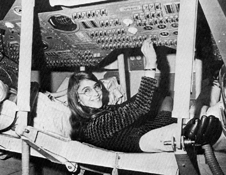
\includegraphics[scale=.6]{img/margaret-in-action.png}      

      \vfill
      {\tiny Fonte: \href{https://en.wikipedia.org/wiki/File:Margaret_Hamilton.gif}{NASA}}
  
  \end{column}
\only<2>{
    \begin{column}{.5\textwidth}
      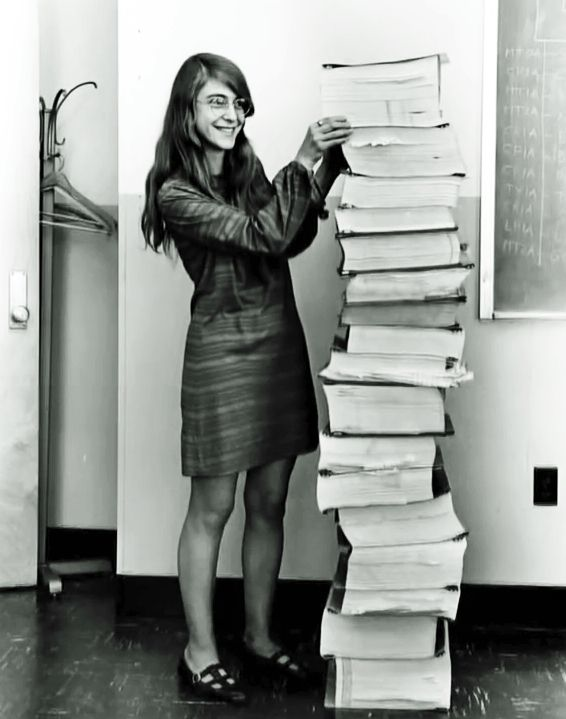
\includegraphics[scale=.22]{img/margaret.png}

      \vfill
      {\tiny Fonte: NASA via \href{https://en.wikipedia.org/wiki/File:Margaret_Hamilton.gif}{Wikipedia}}      
    \end{column}
}
  \end{columns}

\end{frame}

\begin{frame}{Referências}
  \begin{thebibliography}{1}

  \bibitem{brooks1975}
    Frederick~{P.}\ Brooks.
    \newblock {\em The Mythical Man-Month}.
    \newblock Addison-Wesley, 1975.
    
  \bibitem{humble:dijkstra1972}
    Edsger~W. Dijkstra.
    \newblock The humble programmer.
    \newblock {\em Communication of the ACM}, 15(10):859--866, 1972.

  \end{thebibliography}

\end{frame}

%% 
% Local variables:
% mode: latex
% mode:auto-fill
% TeX-file: main
% End:
%%

%% Fonte: http://users.csc.calpoly.edu/~jdalbey/205/Lectures/myths.html

\lecture{Mitos de Desenvolvimento de Software}{myths}

\lecturetitle{\course}{\insertlecture}

\section*{\insertlecture}

\frame{\maketitle}

\begin{frame}{Mítico Homêm-Mês}
\footnotesize
  \begin{columns}
    \begin{column}{.4\textwidth}
      
\includegraphics[scale=.35]{img/mitico.png}
    \end{column}
    \begin{column}{.6\textwidth}
      \begin{itemize}
      \item Observações do autor sobre a experiência de desenvolvimento 
        do sistema operacional OS/360 (1964--*) na IBM.
      \item 1$^a$ publicação: 1975.
      \end{itemize}
    \end{column}

  \end{columns}
  
\end{frame}

\begin{frame}{\inserttitle}

Os mitos são classificados de acordo com o ponto de vista de quem 
os emprega em mitos de:

  \begin{enumerate}[<+-| alert@+>]
  \item Gerenciamento;
  \item Desenvolvimento;
  \item Desenvolvedor.
  \end{enumerate}

\end{frame}

\note{A seguir são descritos alguns mitos que normalmente conduzem à
produção de software com defeitos, atraso na entrega ou cancelamento
do projeto. Os mitos foram classificados de acordo com o ponto de
vista de quem os emprega.}

\begin{frame}{Mitos de Gerenciamento}
\small
\begin{description}[<+-| alert@+>]
\item[Normas e padrões] Normas são editadas por empresas e comitês, às
  vezes são úteis. Porém, podem se tornar irrelevantes, incompletas e
  incompreensíveis se não estiverem vinculadas à realidade.
\item[Ferramentas] Ferramentas podem ajudar, porém não fazem mágica. A
  solução de problemas requerem mais que ferramentas, requerem um
  profundo entendimento do problema e da solução. Segundo Fred
  Brooks~\cite{brooks1975}, não há ``bala de prata'' no
  desenvolvimento de software.
\item[Mais programadores:] A solução intuitiva de que adicionando mais
  programadores pode fazer com que um projeto cumpra seu prazo é
  completamente errônea. Este procedimento causa sobrecarga de
  comunicação e atraso devido ao tempo que os novos integrantes da
  equipe leva para entender o problemas e solução. Segundo Fred
  Brooks~\cite{brooks1975}, ``adicionando pessoas a um projeto
  atrasado torna-o mais atrasado''.
\end{description}

\end{frame}

\begin{frame}{Mitos de Desenvolvimento}

\begin{description}[<+-| alert@+>]
\item[Alterações são fáceis:] Alterações em um software não são
  facilmente acomodadas como a princípio parecem ser. As alterações
  podem tornar o software mais complexo, introduzir novos erros e
  exigir uma quantidade enorme de trabalho devido às modificações em
  todos os processos relacionados (teste, documentação, $\ldots$).

\item[Visão superficial:] {\bf Uma visão geral da solução é suficiente
    para começar a programar.} É necessário um visão concreta sobre os
  requisitos, para detalhar os problemas e soluções para dar início ao
  desenvolvimento.
\end{description}

\end{frame}

\begin{frame}{Mitos do Desenvolvedor}

\begin{itemize}[<+-| alert@+>]
\item {\bf O trabalho acaba quando o programa é entregue:} O software requer
  atenção após a entrega, a manutenção, aperfeiçoamento e extensões
  geram uma necessidade contínua de suporte.
\item {\bf O sucesso de um projeto depende somente da qualidade do software
  entregue:} Documentação e informações de configuração são
  extremamente importantes.
\item {\bf Não há como avaliar a qualidade de um software até que ele
  esteja executando:} Devido a natureza abstrata do software, ele pode
  ser avaliado sem que uma linha de código seja produzida. Há métodos
  formais de análise para verificação de pontos críticos com relação à
  corretude, segurança e confiabilidade.
\end{itemize}

\end{frame}

\begin{frame}{Referências}
\bibliographystyle{plain}
\bibliography{software-engineering}
\end{frame}


%%
% Local variables:
% mode: latex
% mode:auto-fill
% TeX-file: main
% End:
%%

%\lecture{Metodologias de Desenvolvimento de Software}{methods}

\lecturetitle{\course}{\insertlecture}

\frame{\maketitle}

\section{Princípios da Engenharia de Software}

\begin{frame}{Princípios de desenvolvimento de software/sistemas}

  \begin{description}[<+-| alert@+>]
  \item[Formalização:] aplicação de métodos formais para aumento da
    confiabilidade;
  \item[Abstração:] representação do mundo real com nível de
    detalhamento adequado para eliminação da complexidade;
  \item[Decomposição:] divisão em partes menores para redução 
    da complexidade;
  \item[Generalização:] descoberta ou adoção de princípios
    fundamentais que permitem reutilização;
  \item[Flexibilização:] adaptação è evolução, extensão e
    aperfeiçoamento.
  \end{description}
  
\end{frame}

\section{Ciclo de vida do software}
  
\begin{frame}{Ciclo de vida do software}

\begin{tikzpicture}
  [cycle/.style={text centered,text width=2.75cm,minimum width=2cm,
    minimum height=1.5cm,draw},every path/.style={->,>=latex,draw}]
  \def\D{2cm}

  \node<1->[cycle,blue] (spec) {Levantamento e Análise de Requisitos};
  \node<2->[cycle,green!40!black] (proj) [below of=spec,yshift=-\D] {Projeto: Especificação, Modelagem};
  \node<3->[cycle] (dev) [right of=proj,xshift=3.25*\D] {Implementação e Testes};
  \node<4->[cycle,red] (deploy) [above of=dev,yshift=\D] {Implantação e Validação};
  \node<5->[cycle,brown] (maintain) [left of=deploy,xshift=-1.15*\D] {Manutenção};
  
  \path<2-> (spec) -- (proj);
  \path<3-> (proj) -- (dev);
  \path<4-> (dev) -- (deploy);
  \path<5-> (deploy) -- (maintain);
\end{tikzpicture}

%%
% Local variables:
% mode: latex
% End:
%%

\end{frame}


\begin{frame}{Desenvolvimento em Cascata}

\begin{tikzpicture}
  [font={\tiny\bf},node distance=2.25cm,every path/.style={->,>=latex,draw},
  cycle/.style={thick,rounded corners=3mm,text centered,text width=1.5cm,minimum width=1cm, minimum
    height=1.5cm,draw},
  dev/.style={cycle},
  deploy/.style={cycle,red},
  maintain/.style={cycle,brown!40!black}]

  \node<1->[cycle,blue] (requirements) {Levantamento e Análise de Requisitos};
  \node<2->[cycle,green!40!black] (proj) [right of=requirements,yshift=-1cm] {Projeto: Especificação, Modelagem};
  \node<3->[dev] (dev) [right of=proj,yshift=-1cm] {Implementação e Testes};
  \node<4->[deploy] (deploy) [right of=dev,yshift=-1cm] {Implantação e Validação};
  \node<5->[maintain] (maintain) [right of=deploy,yshift=-1cm] {Manutenção};
  
  \path<2-> (requirements) edge [bend left] (proj.north);
  \path<3-> (proj) edge [bend left]  (dev.north);
  \path<4-> (dev) edge [bend left]  (deploy.north);
  \path<5-> (deploy) edge [bend left]  (maintain.north);
\end{tikzpicture}
  

\end{frame}

\begin{frame}{Método Evolutivo}
  \begin{center}
  \begin{tikzpicture}
    [font=\scriptsize,phase/.style={minimum height=1cm,draw},
    protophase/.style={minimum width=3cm,ellipse,draw},
    version/.style={white,fill=black,circle,draw},
    every path/.style={->,>=latex,draw}]

    \node[phase,tape,thick] (requirements) {Requisitos};
    \node[thick,minimum height=5cm,minimum width=3.2cm,draw] (prototype) [right of=requirements,xshift=2cm] {};
    \node[above] at (prototype.north) {Prototipação};
    \node[fill=yellow,protophase] (dev) [right of=requirements,xshift=2cm,yshift=1cm]
    {Implementação};
    \node[fill=gray,protophase] (eval) [right of=requirements,xshift=2cm,yshift=-1cm]  {Validação};
    
    \node[version] (v0) [right of=prototype,xshift=2cm,yshift=2.5cm] {Versão
      0};
    \node[version] (v1) [right of=prototype,xshift=2cm]
    {Versão 1};
    \node[]  [right of=prototype,xshift=2cm,yshift=-1.25cm] {$\vdots$};
    \node[version] (vN) [right of=prototype,xshift=2cm,yshift=-2.5cm] {Versão N};

    \path (requirements) -> (prototype);
    \path (dev.south west) -> (eval.north west);
    \path (eval.north east) -> (dev.south east);
    \path (prototype.north east) -> (v0);
    \path (prototype.east) -> (v1);
    \path (prototype.south east) -> (vN);
  \end{tikzpicture}
\end{center}

\end{frame}


\begin{frame}{Método Evolutivo}

\begin{block}{Vantagens}
  \begin{itemize}[<+-| alert@+>]\setbeamercovered{transparent}
  \item Verificação antecipada de possíveis problemas durante a
    implementação: linguagem de programação, algoritmo, performance.
  \item Maior interação com o cliente, permitindo esclarecer dúvidas
    sobre requisitos que não estejam bem definidos.
  \end{itemize}
\end{block}  

\end{frame}

\begin{frame}{Método Evolutivo}

\begin{block}{Desvantagens}
  \begin{itemize}[<+-| alert@+>]\setbeamercovered{transparent}

    \item Não é dada atenção à documentação, pois cada protótipo é
      visto como provisório.

  \item Pode causar inconsistências na estrutura do projeto.
    \note{Envolve o mito de que alterações são fáceis}

    \item Dá a impressão ao cliente, em algumas versões, de que o
      projeto está quase pronto.
      \note{O cliente irá pressionar para usá-lo, achando que somente
        algumas alterações são necessárias}

    \item O desenvolvedor pode fazer escolhas inapropriadas para
      adiantar um protótipo, prejudicando as versões seguintes.
  \end{itemize}
\end{block}

\end{frame}


\begin{frame}{Método Espiral}{Boehm}
  
  \begin{block}{Características}
    \begin{itemize}[<+-| alert@+>]\setbeamercovered{transparent}
    \item Incorpora características dos processos em cascata e
      evolutivo, com a adição da análise de risco.
      \note{Dá atenção especial às partes críticas do projeto}
    \item Cada iteração da espiral se beneficia das lições da anterior.
    \item O protótipo está mais voltado para o projeto e não para o
      funcionamento do sistema.
      \note{Evita expectativas do cliente com relação ao programa.}
      \item Mais flexível que o cascata;
      \item O protótipo não é funcional, o que provoca riscos em caso
        de pressão para produzir algo ou corte de gastos;
    \end{itemize}
  \end{block}
\end{frame}


\begin{frame}{Método Espiral}

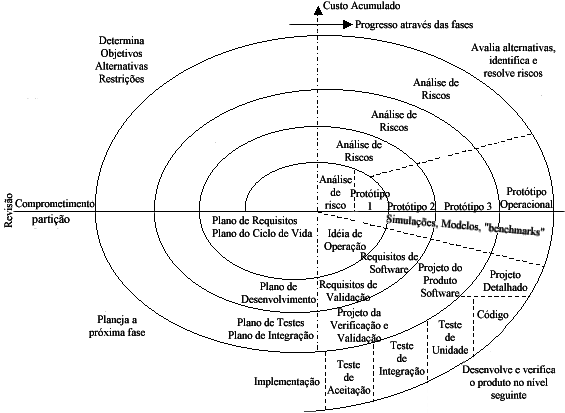
\includegraphics[scale=.4]{img/spiral.png}

\vfill
{\tiny Fonte: \href{http://www2.dem.inpe.br/ijar/CicoloVidaSoftPrado.html}{Engenharia de Software, Capítulo 2 - Ciclo de Vida do Software, Professor Prado.}}
\end{frame}


\lecture{Rational Unified Process (RUP)}{RUP}

\begin{frame}{\insertlecture}
  Processo baseado na UML ({\em Unified Modeling Language}) criado
  pela Rational Corp., adquirida pela IBM. O processo baseia-se nas
  fases conforme a figura a seguir:

  \begin{center}
    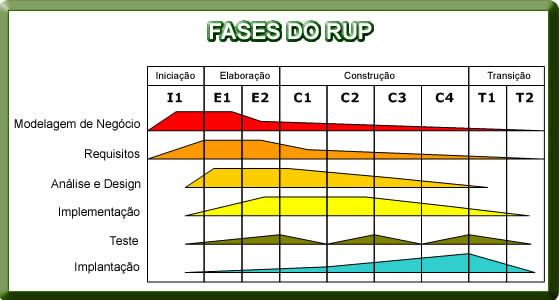
\includegraphics[scale=.6]{img/fasesRUP.png}\\
    {\tiny Fonte: \href{https://www.infoescola.com/engenharia-de-software/rup/}{RUP. Marina Martinez.}}
  \end{center}
\end{frame}

\begin{frame}{\insertlecture}{Fases}
  \begin{enumerate}[<+-| alert@+>]\setbeamercovered{transparent}
  \item {\bf Concepção/Iniciação}: define o escopo do projeto,
    cronograma e despesas. É usado para verificar o progresso.
  \item {\bf Elaboração}: trabalho com o cliente para identificar
    casos de uso, projeta a arquitetura de software, ajusta o plano de
    desenvolvimento e constrói um protótipo inicial.
  \item {\bf Construção}: codifica e testa o produto, resultando no
    primeiro lançamento de teste.
  \item {\bf Transição}: move o produto do ambiente de desenvolvimento
    para o ambiente de produção, onde inclui o teste de aceitação do
    cliente e o treinamento do usuário.
  \end{enumerate}
\end{frame}

\begin{frame}{\insertlecture}{\em Workflows}
  \begin{enumerate}[<+-| alert@+>]\setbeamercovered{transparent}
  \item Modelagem de negócio;
  \item Requisitos;
  \item Análise e especificação/design;
  \item Implementação;
  \item Teste;
  \item Implantação.
  \end{enumerate}
\end{frame}

\begin{frame}{\insertlecture}{Considerações}
  \begin{itemize}
  \item Diferente do Cascata, cada fase do RUP envolve iteração. Por
    exemplo, a concepção pode ter uma iteração, a elaboração duas, a
    construção quatro e a transição duas. Como o Espiral, o RUP pode
    iterar através das quatro fases repetidamente.
  \end{itemize}  
\end{frame}

\begin{frame}{Abordagem de Planejar-Documentar}
  \begin{itemize}[<+-| alert@+>]\setbeamercovered{transparent}
  \item O métodos e processos vistos exigem uma abordagem
    que envolve Planejamento e documentação, por isso, são considerados
    mais pesados do que as abordagens Ágeis.
  \item Alguns programadores consideram estas metodologias tediosas 
    para o desenvolvimento de software.
  \end{itemize}
\end{frame}

% \begin{frame}{Métodos ágeis}
  
%   \begin{block}{Características}
%     \begin{itemize}[<+->]
%     \item Código como principal medida de progresso;
%     \item Colaboração entre desenvolvedores e clientes que participam
%       mais ativamente das fases de desenvolvimento;
%     \item Comunicação frequente;
%     \item Simplificação da documentação;
%     \item Testes como guias para o desenvolvimento;
%     \item Desenvolvimento em pequenos incrementos com integração contínua;
%     \item Práticas como programação em grupos de duas pessoas.
%       \note{Para aumentar o número de pessoas pensando sobre as
%         decisões técnicas e capturar erros mais facilmente.}
%     \end{itemize}
%   \end{block}
% \end{frame}


\begin{frame}{Referência}
  \begin{itemize}
  \item {\color{blue}''Engineering Software as a Service: An Agile Approach Using
    Cloud Computing.''} Armando Fox,‎ David Patterson. Strawberry Canyon
    LLC, 2014.
  \end{itemize}  
\end{frame}
%\lecture{Levantamento e Análise de Requisitos}{requirements}

\lecturetitle{\course}{\insertlecture}

\section{\insertlecture}

\frame{\maketitle}

\begin{frame}{\insertlecture}
  
  \begin{itemize}[<+->]\setbeamercovered{transparent}
  \item O software deve se adaptar às necessidades dos usuários;
    \begin{itemize}
    \item As melhores técnicas de programação---algoritmos, estrutura de dados, 
      análise de performance, estrutura modular---não salvarão o projeto da falha.
    \end{itemize}
  \item Os softwares são construídos para atender os clientes, em especial os usuários, 
    e devem se adaptar às suas necessidades.
  \end{itemize}

  \pause
  
  O levantamento e análise de requisitos tenta atingir um equilíbrio
  entre o que os usuários querem e o que o sistema fará.
  \note{Equilíbrio porque alguma negociação deve haver.}

\end{frame}

\begin{frame}{Produtos da fase requisitos}
  \begin{description}[<+->]\setbeamercovered{transparent}
  \item[Documento de requisitos] descrevendo as características do
    software a ser construído.
  \item[Plano de validação] descrevendo como o futuro software, uma
    vez construído, será testado.
  \end{description}
\end{frame}

\begin{frame}{O Padrão IEEE}
  \begin{itemize}
  \item
    \href{http://holanda.xyz/files/720574.pdf}{Prática
      Recomendada para as Especificações de Requisitos de
      Software. IEEE Computer Society. IEEE Std 830-1998.}

    \begin{itemize}
    \item Conjunto de listas para checagem de propriedades que o sistema
      deve satisfazer.
    \end{itemize}
    \note{O padrão ajuda a levantar as propriedades, tentando antecipar
      problemas que poderiam ocorrer.}
  \end{itemize}
\end{frame}

\begin{frame}{Escopo dos Requisitos}
  \begin{description}[<+->]\setbeamercovered{transparent}
  \item[Requisitos Funcionais] definem as funções que o sistema deve
    possuir. Possuem entrada, processamento e saída.
  \item[Requisitos Não-Funcionais] performance, portabilidade, éticos,
    legais, integração.
  \end{description}
\end{frame}

\begin{frame}{Obtendo os Requisitos}
  
  A obtenção dos requisitos é uma {\bf negociação} entre as propriedades
  desejadas pelo usuário para o sistema e as possibilidades de
  desenvolvimento e custos expostas pela equipe técnica.

  \pause

  \begin{block}{Principais fatores a serem equilibrados}
  \begin{itemize}[<+->]\setbeamercovered{transparent}
  \item Alguns usuários têm visões conflitantes sobre o sistema;
  \item Algumas propriedades desejadas são inviáveis em termos de custo ou 
    desenvolvimento;
  \item Os usuários tendem a pensar em termos de sistemas existentes;
  \item Fatores externos afetam a escolha das funcionalidades,
    principalmente, custo e interferência da instituição onde o
    sistema será implantado.
  \end{itemize}
\end{block}

\end{frame}

\begin{frame}{Técnicas para levantamento de requisitos}
  \begin{itemize}[<+->]\setbeamercovered{transparent}
  \item Entrevistas;
  \item Workshops;
  \item Sistemas anteriores;
  \item Sistemas similares.
  \end{itemize}
\end{frame}

\frame{\author{}\date{}\title{Documentação de requisitos}\maketitle}

\subsection{Documentação de requisitos}

\begin{frame}{Documentação dos requisitos}
  Formas de escrever uma especificação de requisitos do sistema:

  \begin{description}[<+->]\setbeamercovered{transparent}
  \item[Sentenças em linguagem natural:] Os requisitos são escritos em forma de frases.
  \item[Linguagem natural estruturada:] Os requisitos são escritos em um formulário.
    \item[Notações gráficas:] Utiliza figuras e diagramas com texto associado.
  \item[Especificações matemáticas:] Usa notações matemáticas, como máquina de estados 
    finitos e teoria de conjuntos.
  \end{description}
\end{frame}

\begin{frame}{Sentenças em linguagem natural}
  Exemplo de requisitos funcionais de um sistema de gestão de pessoas, disciplinas e notas 
  de uma Faculdade ou Universidade:
  \begin{enumerate}
  \item Cadastro de pessoas por funcionários da Faculdade.
    \item Consulta de pessoas por funcionários da Faculdade.
    \item Cadastro de disciplinas por funcionário da Faculdade. 
    \item Inserção de notas por professores.
    \item Consulta de notas por parte dos alunos.
    \end{enumerate}
\end{frame}

\begin{frame}{Linguagem natural estruturada}

  {\bf Sistema de gerenciamento para Faculdade ou Universidade}\\\bigskip

  \begin{tabular}[h]{|l|l|}\hline
    \bf Função: & Gerenciar dados de pessoas, disciplinas e notas.\\\hline
    \bf Descrição: & O sistema deve armazenar os dados de funcionários, \\
    & alunos e docentes, de disciplinas e de notas.\\\hline
    \bf Entradas: & Pessoas: nome, endereço, RG, CPF.\\
                & Disciplinas: nome, responsável, resumo.\\
                & Notas: nome da disciplina, nome do aluno, valor.\\\hline
    \bf Saídas: & Visualização das entradas.\\\hline
    
  \end{tabular}
\end{frame}

\begin{frame}{Notação gráfica}
  
  Exemplo de uso de notação gráfica para a documentação de requisitos, no 
  caso, diagrama de casos de uso da UML ({\em Unified Modeling Language}):

  \begin{center}
    \includegraphics[scale=.35]{usecase.png}
  \end{center}

\end{frame}

\begin{frame}{Especificações matemáticas}
  
  Especificação do sistema de uma catraca usando máquina de estados finitos:\bigskip
\begin{center}
  \includegraphics[scale=.35]{state.png}
\end{center}
\end{frame}

\begin{frame}[fragile]{Especificações matemáticas, continuação}

  Especificação de um relógio binário usando a lógica temporal de ações (TLA$^+$, \href{http://research.microsoft.com/en-us/um/people/lamport/tla/tla.html}{\em Temporal Logic of Actions}):

\begin{multline}
  \text{VARIABLE clock}\hfill\\
  \text{Init} \equiv clock \in \{0, 1\}\hfill\\
  \text{Tick} \equiv \text{IF}\ clock = 0\ \text{THEN}\ clock' = 1\ \text{ELSE}\ clock' = 0\hfill\\
  \text{Spec} \equiv \text{Init} \land [][\text{Tick}]_{\langle clock\rangle}\hfill
\end{multline}

\end{frame}

\begin{frame}{Referências}  
  \begin{enumerate}
  \item \ianref
  \item \pfref
  \item Bertrand Meyer, ``Touch of Class: Learning to Program Well
    with Objects and Contracts'', Springer, 2009.
  \end{enumerate}
\end{frame}
%\input viabilidade
\input project
%\input uml
%\input classes
%\input inheritance
%\input polymorphism
%\input generics

%\input quality
%\input cmmi
%\input spice
%\input metricas
\input agil

\input config
\input vcs
\input make
\input TDD
%\input refactoring
%\input formal
%\input tlaplus
\end{document}
